\chapter{Zug}
\section{Funktionsweise}

Aufgrund der Verlagerung der Logik auf den Raspberry Pi ist die Funktionsweise des Zuges sehr beschränkt.\\
Beim Start der Zugsoftware wird zuerst eine langsame Fahrt des Zuges durchgeführt um mithilfe des als nächstes gelesenen Tag die Position des Zuges zu bestimmen. Diese wird nun an den Raspberry Pi übermittelt und die Antwort abgewartet. Die nun empfangene Anweisung wird durchgeführt, was bedeutet das die Werte für "beforeSpeed", "tag" und "afterSpeed" ausgelesen und abgespeichert werden. "beforeSpeed" wird zusätzlich als aktuelle Geschwindigkeit gesetzt.\\
Wird nun während der Ausführung der Anweisung ein neuer Tag gelesen wird dieser mit dem Wert aus "tag" verglichen. Sollte sich der gelesene Tag von dem gespeicherten unterscheiden hält der Zug an. Ansonsten wird "afterSpeed" als neue Geschwindigkeit gesetzt. In jedem Fall wird der gelesene Tag erneut an den Raspberry Pi übermittelt.\\
Abgesehen von der Socket-Verbindung (Beschrieben in Kapitel \ref{chap:socket}) wurde keine weitere Logik für den Zug implementiert.

\section{Merging der Projekte in ein Projekt}
\begin{figure}
	\caption{Aufbau der Projekte. Rechts das alte, links das neue Projekt}
	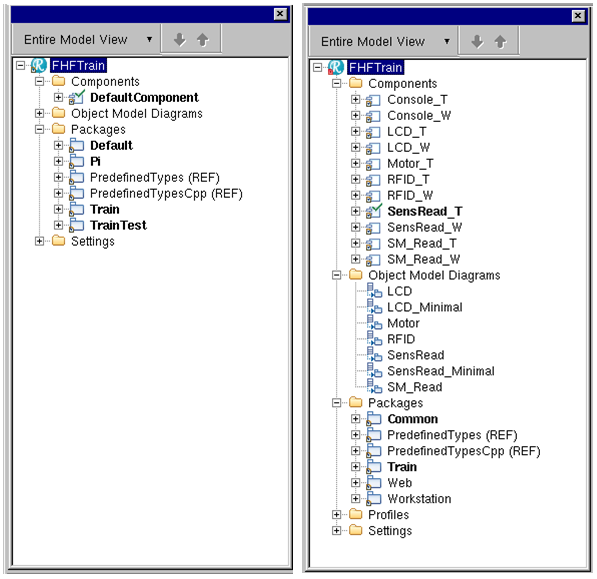
\includegraphics[width=1\textwidth]{content/pictures/train/structure.png}
	\label{pic:train_structure}
\end{figure}
Das FHFTrain-Projekt basiert auf dem Semesterprojekt des Sommersemesters 2016. Der Code, der den Zug grundsätzlich zum Fahren bringt und die Hardware ansteuert, muss also zusammen mit dem neuen Code, also Algorithmus und Socket, "gemerged" werden. In Abbildung \ref{pic:train_structure} sieht man zunächst den jeweils grundgelegenen Aufbau der beiden Projekte.\\  
Das alte Semesterprojekt beinhaltet mehrere Components, die jeweils mit T oder W beschriftet sind, für Train und Workstation.\\
Das aktuelle Projekt beinhaltet nur eine Component und mehreren Packages, jeweils für den Raspberry Pi (Als Pi bezeichnet) und den Zug (Als Train bezeichnet). Zusätzlich gibt es noch ein Testpackage, TrainTest.\\
Zunächst wird das alte Projekt geöffnet, über \textit{File->Insert Project->Existing…} lässt sich ein zweites Projekt in die Modelübersicht aufnehmen. Danach können sowohl Components, als auch Diagramme und Packages per \textit{Ctrl+Drag} übertragen werden. In der finalen Version wird die "DefaultComponent" aus dem aktuellen Projekt in die Components "Algorithm\_Socket" und "Train\_Socket" aufgeteilt. "Algorithm\_Socket" verwaltet dabei den kompletten Algorithmus und die Socket-Verbindung auf dem Pi. "Train\_Socket" hingegen ist für die Kommunikation auf dem Zug zuständig, diese Component verwaltet also, was an den Pi geschickt wird und wie die Informationen gehandhabt werden sollen, die vom Pi ankommen.\\
In Abbildung \ref{pic:train_structure_merged} ist die vollständige Modellübersicht des gemergten Projektes zu sehen.
\begin{figure}
	\caption{Aufbau des Projektes nach dem Merge}
	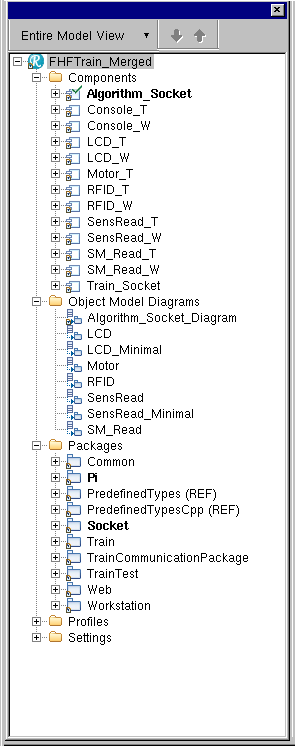
\includegraphics[height=0.8\textheight]{content/pictures/train/structure_merged.png}
	\label{pic:train_structure_merged}
\end{figure}

\section{Zusammenführung des Codes}

Nachdem beide Projekte „gemerged“ worden sind, müssen noch mehrere Stellen im Code modifiziert werden.\\
Im ersten Schritt wird eine Verbindung zwischen der Train-Kommunikation und der Shared-Memory aufgebaut. Die Shared-Memory steht allen Komponenten des Zuges zur Verfügung, über diese können die Komponenten Daten austauschen. In der Shared-Memory werden Datentypen für AfterSpeed und BeforeSpeed erstellt, also die Geschwindigkeiten, die der Zug bis zu einem Tag und ab einem Tag fahren soll.\\
Als nächstes wird eine Methode implementiert, die die Befehle des Pis in Substrings unterteilen und die Geschwindigkeiten in die Shared-Memory eintragen. Die Motor-Komponente sorgt dann automatisch dafür, dass die neue Geschwindigkeit gefahren wird.\\
Im letzten Schritt muss noch dafür gesorgt werden, dass der Zug dem Pi auch seine Position mitteilen kann. Dazu wird eine Funktion implementiert, die immer, wenn der Zug einen RFID Tag erkennt, einen dazugehörigen float-Wert in die Shared-Memory speichert. Schließlich wird noch implementiert, dass der TrainSpeaker genau dann seine Position an den Pi sendet, wenn in der Shared-Memory eine Änderung des RFID-Tags stattgefunden hat.\\
Nach diesen Arbeitsschritten sind die beiden Projekte endgültig  zu einem Projekt „gemerged“, welches dann auch funktionstüchtig ist.
